\section{Теоритические сведения}
\subsection{Принцип работы оптических приборов}
Оптические приборы, в которых осуществляется физическое разложение электромагнитного излучения на монохроматические составляющие, называются спектральными. Спектральный состав электромагнитного излучения может много рассказать о своём источнике и осреде, в которой излучение распространялось. Существуют сотни приборов, анализирующих спектры ---  от радиодиапазона до высокоэнергетических $\gamma$-квантов. По характеру распределения интенсивности в спектральном разложении спектры могут быть разделены на линейчатые (например, спектры излучения атомов), непрерывные или сплошные (например, спектр излучения абсолютно чёрного тела), а также смешанные, представляющие собой наложение линейчатых и непрерывных спектров (например, спектр излучения Солнца). В данном лабораторном практикуме наблюдение спектров проводится на установках, основными элементами которых являются дифракционная решётка, интерферометр Фабри–Перо и призма.  Эти установки позволяют проводить визуальное наблюдение линейчатых спектров, состоящих из набора узких спектральных линий в оптическом диапазоне длин волн, и на них можно довольно точно определить значение длины волны, но интенсивность спектральной линии определяется грубо, <<<на глаз>>>.

\begin{figure}[ht!]
    \center{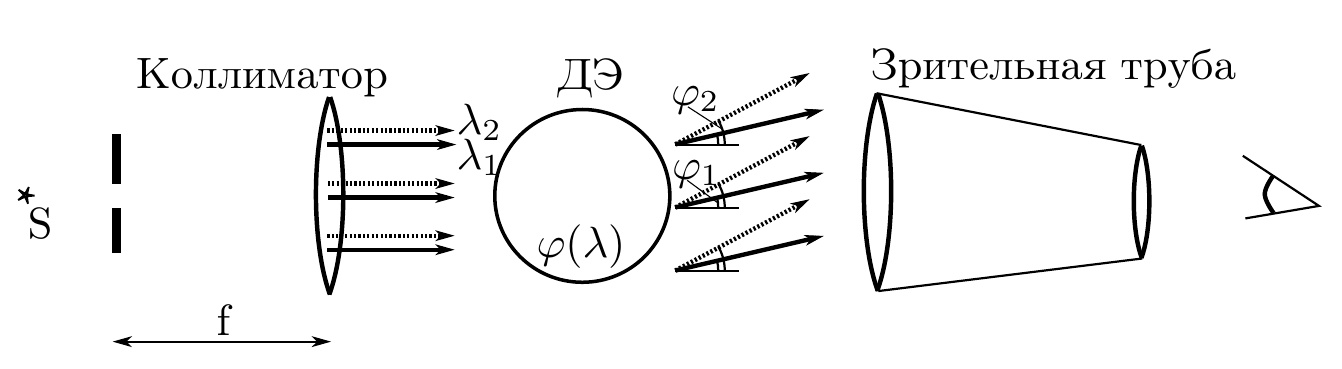
\includegraphics[width=0.8\linewidth]{../img/th1.png}}
\end{figure}

Принципиальная схема установки для изучения спектров приведена на рисунке. Свет от источника S попадает на экран, в котором имеется отверстие в виде щели. Экран располагают в фокальной плоскости линзы или системы линз. Коллиматор формирует пучок света, близкий к параллельному. После коллиматора пучок лучей попадает на диспергирующий элемент (ДЭ): амплитудную или фазовую дифракционную решётку, интерферометр Фабри–Перо или призму. Наблюдаются изображения с помощью зрительной трубы, установленной на бесконечность. Если удалить из схемы диспергирующий элемент, а коллиматор и зрительную трубу расположить на одной оси, то можно увидеть чёткое изображение входной щели коллиматора.

Диспергирующий элемент перераспределяет интенсивность падающего на него излучения по углам в зависимости от длины волны: каждой монохроматической компоненте излучения с длиной волны $\lambda$ соответствует один или несколько углов $\varphi(\lambda)$ на выходе прибора, в направлении которых интенсивность прошедшей волны максимальна. Иными словами, диспергирующий элемент пространственно разделяет монохроматические составляющие падающего на него излучения, осуществляя тем самым его физическое разложение по спектру. При известной зависимости $\varphi(\lambda)$ по измеряемому углу поворота $\varphi$ зрительной трубы можно определить длину волны спектральной линии.

Каждый спектральный прибор предназначен для решения конкретной задачи спектроскопии. Выбор прибора для исследования спектра какого-либо источника должен заключаться в сравнении его характеристик с требуемыми. Наиболее важными характеристиками являются угловая дисперсия, разрешающая способность и дисперсионная область.

Разрешающая способность $R = \frac{\lambda}{\delta\lambda}$ характеризует возможность прибора различать две близкие спектральные линии с длинами волн $\lambda$ и $\lambda + \delta\lambda$

Угловая дисперсия $D = \frac{d\varphi}{d\lambda}$~--- производная зависимости угла отклонения $\varphi(\lambda)$ волны диспергирующим элементом по $\lambda$. По величине угловой дисперсии можно определить угловое расстояние между двумя близкими спектральными линиями: $\delta\varpi\approx D\delta\lambda$.

Дисперсионная область (или область дисперсии)~--- предельная ширина спектрального интервала $\Delta\lambda$ прибора, для которой дифракционные максимумы соседних порядков не перекрываются. Она определяет диапазон длин волн, при которых прибор может быть использован для анализа спектра.

\subsection{Дифракция}
Дифракцией называются отклонения в распространении волн от законов геометрической оптики.

Основными параметрами, определяющими характер дифракционных явлений, является длина волны $\lambda$, размер отверстия $b$ и расстояние до плоскости наблюдения $z$. Характер дифоракции определяется волновым параметром

\[
    p = \frac{\sqrt{\lambda z}}{b}
\]

При $p \ll 1$ выполняются законы геометрической оптики, при $p\approx 1$ происзодит дифракция Френеля, $p\gg 1$~--- дифракция Фраунгофера.

\subsection{Принцип Гюйгенса-Френеля}
\begin{figure}[ht!]
    \center{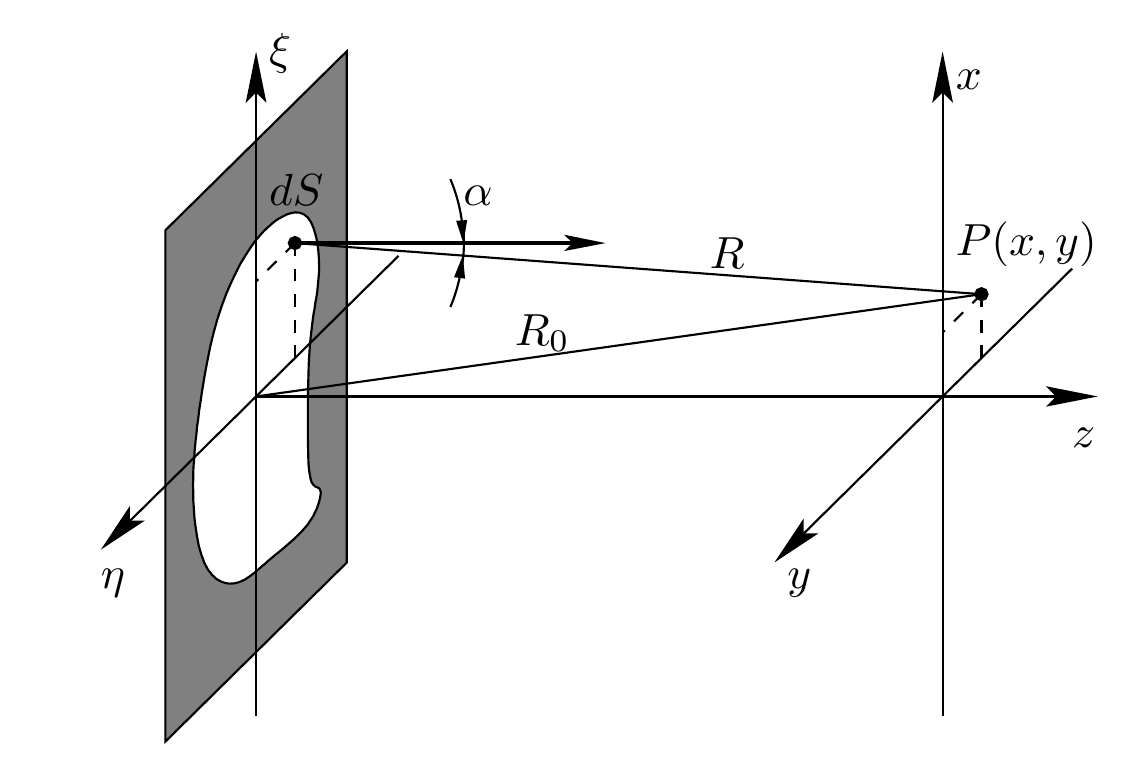
\includegraphics[width=0.8\linewidth]{../img/gufr.png}}
\end{figure}

Пусть волна света, созданная источниками, расположенными в области $z < 0$, достигла плоскости $z=0$. Световое поле в этой плоскости нам известно. Пусть его комплексная амплитуда есть
\[
    f_{0}(x, y) = a_{0}(x, y)e^{i \varphi_{0}(x, y)}
\]
где функции $a_{0}(x, y)$ и $ \varphi_{0}(x, y)$ описывают распределение амплитуд и фаз колебаний в плоскости $z=0$.

Согласно принципу Гюйгенса, каждую точку $( \xi, \eta)$ плоскости $z = 0$, куда пришла волна, можно рассматривать  как источник вторичной волны. То есть можно представить себе, что волна возбуждает колебания некоторого фиктивного источника (осциллятора), который и переизлучает вторичную волну. Частота $ \omega$ этой переизлучённой волны совпадает с частотой исходной монохроматической волны. Френель дополнил принцип Гюйгенса, предложив рассматривать световое колебание в любой точке наблюдения в области $z > 0$ как результат интерференции этих вторичных волн.

Предполагается, что амплитуда излучения вторичного источника пропорциональна амплитуде $a_{0}(\xi, \eta)$  колебания, созданного реальной волной, пришедшей к площадке $ds$. Фаза колебания также задаётся фазой $ \varphi( \xi, \eta)$ пришедшей к элементу $ds$ волны.

Далее предполагается, что маленькая площадка $ds$ переизлучает, подобно точечному источнику, сферическую волну, т. е. для вычисления вклада, который даёт эта площадка в суммарное колебание в точке наблюдения $P$,  нужно учесть ослабление амплитуды и набег фазы $e^{ikR}/R$. Наконец, предполагается, что амплитуда колебания пропорциональна видимой из точки наблюдения площади элемента $ds$, т.е. пропорциональна $ds\cos\alpha$. Таким образом, вклад элемента $ds$ пропорционален величине
\[
    f_{0}(\xi, \eta)\frac{e^{ikR}}{R}\cos\alpha\cdot d\xi d\eta
\]
Полное световое колебание $g(x, y)$ есть результат интерференции всех вторичных волн, посылаемых всеми площадками $ds$, расположенными в области отверстия:
\[
    g(x, y) = \frac{1}{i\lambda}\iint_{S} f_{0}(\xi, \eta)\frac{e^{ikR}}{R}\cos\alpha d\xi d\eta
\]

При условии, что размер препятствия мал по сравнению с расстоянием $R_{0}$ до точки наблюдения, амплитудный множитель $\frac{1}{R}$,  учитывающий уменьшение амплитуды в сферической волне по мере удаления от вторичного источника $ds$, можно заменить постоянной величиной $\frac{1}{R_{0}}$. Множитель наклона $\cos\alpha$ также считаем приблизительно одинаковым (и равным единице) для всех вторичных источников, расположенных в области отверстия. Тогда в этом приближении принцип Гюйгенса—Френеля приобретает следующий вид:
\[
    g(x, y) = \frac{1}{i\lambda R_{0}} \iint f_{0}(\xi, \eta)e^{ikR} d\xi d\eta
\]
\[
    R \approx z + \frac{\left(x - \xi\right)^{2}}{2z} + \frac{\left(y - \eta\right)^{2}}{2z}
\]

Тогда
\[
    g(x, y) = \frac{e^{ikz}}{i \lambda z}\iint f_{0}(\xi, \eta)e^{i\frac{k}{2z}\left(\left(x-\xi\right)^{2} + \left(y - \eta\right)^{2}\right)} d\xi d\eta
\]
Если отверстиеосвещается плоской волной, то $f_{0}(\xi, \eta) = A_{0}$.

\subsection{Дифракция Фраунгофера}
Рассмотрим дифракцию на отверстии в плоском экране, находящемся в плоскости $z = 0$. Пусть точка наблюдения имеет координаты $P(x, y, z)$. Расстояние $R$  от площадки $ds$ в точке экрана $(\xi, \eta)$ до точки $P$ равно
\[
    R = \sqrt{z^{2} + \left(x - \xi\right)^{2} + \left(y - \eta\right)^{2}}\approx R_{0} - \frac{x\xi + y\eta}{R_{0}} + \frac{\xi^{2} + \eta^{2}}{2R_{0}}
\]
$R_{0} = \sqrt{x^{2} + y^{2} + z^{2}}$~--- расстояние от начала координат $O$ до точки наблюдения.
\[
    \xi^{2} + \eta^{2} \le b^{2} \ll \lambda R_{0}
\]
Тогда последним слагаемым в $R$ можно пренебречь и
\[
    R\approx R_{0} -\frac{x\xi}{R_{0}} - \frac{y\eta}{R_{0}}
\]

Тогда принцип Гюйгенса-Френеля запишется в виде
\[
    g(x, y) = \frac{e^{ikR_{0}}}{i\lambda R_{0}}\iint f_{0}(\xi, \eta)e^{-i\left(\frac{kx}{R_{0}}\xi + \frac{ky}{R_{0}}\eta\right)} d\xi d\eta
\]
В одномерном случае
\[
    g(x) \approx \int_{-\infty}^{+\infty} f_{0}(\xi)e^{-\frac{ikx\xi}{R_{0}}}d\xi
\]
$u = \frac{kx}{R_{0}}$, а картина дифракции Фраунгофера представляет собой преобразование Фурье граничного поля $f_{0}(\xi)$.

\begin{figure}[ht!]
    \center{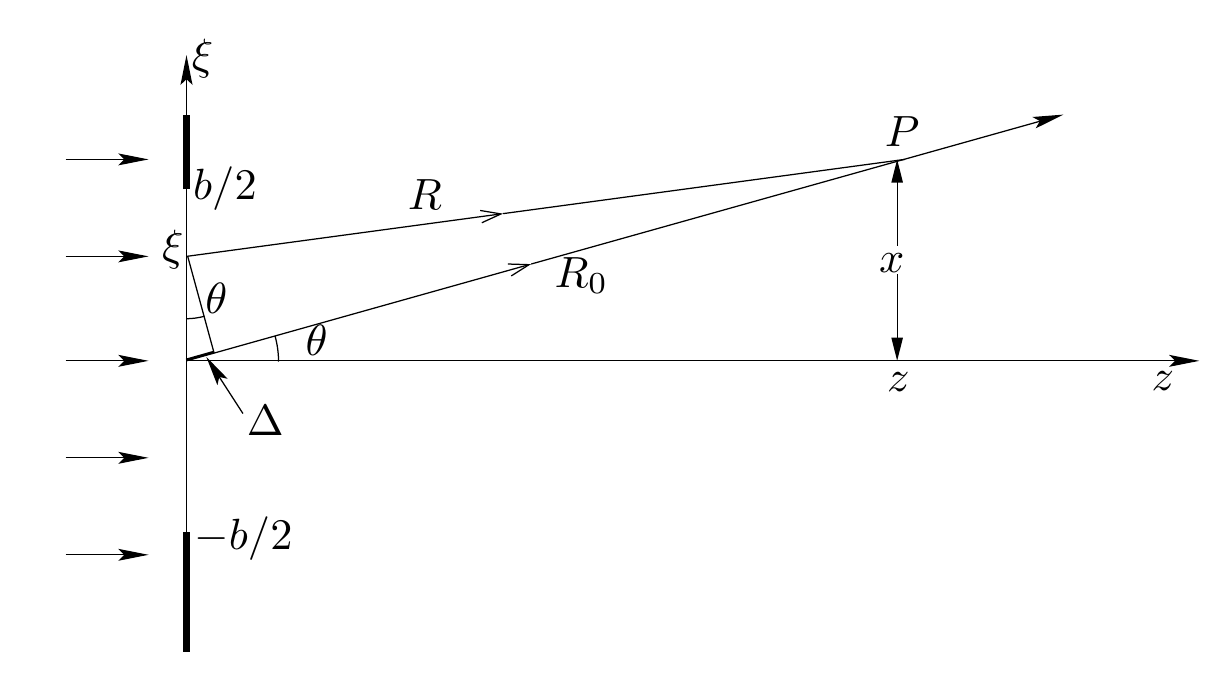
\includegraphics[width=0.8\linewidth]{../img/frau.png}}
\end{figure}

Определим разность хода волн $\Delta$,  приходящих к удалённой точке наблюдения от двух вторичных источников, один из которых находится в точке с координатой $\xi$, а второй — в точке $\xi = 0$. Удалённость точки $P$  позволяет считать направления волн, идущих из этих точек практически параллельными, следовательно, разность их хода равна
\[
    \Delta = \xi \sin \theta
\]
Соответственно разность фаз колебаний равна $ \varphi = -k\xi \sin \theta$, где $ \theta$~--- направление на удалённую точку наблюдения, имеющую координату $x$:
\[
    k\sin \theta = \frac{kx}{R_{0}} = u
\]

Таким образом
\[
    g(u) \approx \int_{-\infty}^{+\infty} f_{0}(\xi)e^{-ik\sin \theta \xi} d\xi
\]

Эта формула~--- полный аналог преобразования Фурье для $f_{0}(t)$
\[
    C(\omega) = \int f_{0}(t)e^{-i\omega t} dt
\]

Эта аналлогия позволяет назвать величину $u=k\sin \theta$ пространственной частотой.

Распределение $I(\theta) \approx g(\theta)$ называется диаграммой направленности.

\subsection{Дифракция Фраунгофера на щели}
Пусть щель шириной $b$ освещается слева плоской нормально падающей волной. Граничное поле $f_{0}(x)$, возникающее в плоскости $z = 0$, примыкающей к непрозрачному экрану со щелью справа, имеет вид прямоугольного выступа шириной $b$. Тогда
\[
    g(\theta) \approx \int_{-b/2}^{b/2} e^{ikx\sin \theta}dx \approx \frac{\frac{kb}{2}\sin \theta}{\frac{kb}{2}\sin \theta}
\]
\begin{figure}[ht!]
    \center{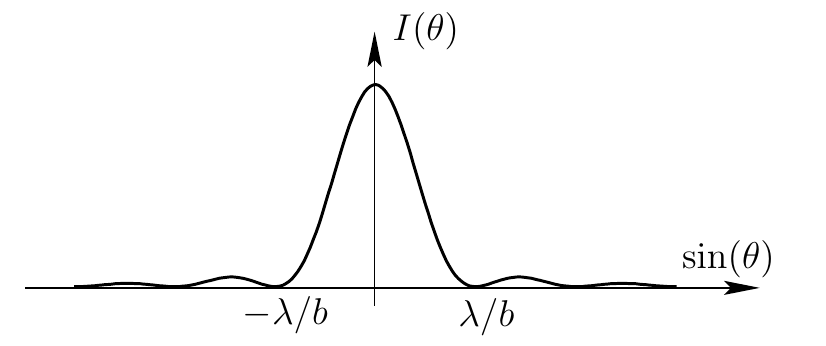
\includegraphics[width=0.8\linewidth]{../img/frau1.png}}
\end{figure}


Почти вся интенсивность $I(\theta) \approx g(\theta)^{2}$ сосредоточена в области
\[
    \left|\sin \theta \right| \le \frac{ \lambda}{b}
\]

\subsection{Дифракция Фраунгофера на двух щелях}
Рядом со щелью, дифракцию на которой мы рассмотрели выше, расположим параллельно ещё одну щель на расстоянии $d$ от первой.

Расстояние от второй щели до точки наблюдения на величину $ \Delta = d\sin\theta$  меньше расстояния между первой щелью и точкой наблюдения. Соответствующая фаза колебания отличается на величину
\[
    \alpha = -k \Delta = -kd \sin \theta
\]
Поэтому колебательный процесс, созданный второй щелью в точке наблюдения, описывается функцией $g( \theta)e^{i \alpha}$.  Волны, посылаемые в точку наблюдения двумя щелями, интерферируют. Амплитуда суммарного колебательного процесса в точке наблюдения есть $g( \theta) + g( \theta)e^{i \alpha}$.

Картина интенсивности
\[
    I( \theta) \approx \left| g( \theta) \right|^{2} \left(1 + \cos \left(kd \sin \theta\right)\right)^{2}
\]

\begin{figure}[ht!]
    \center{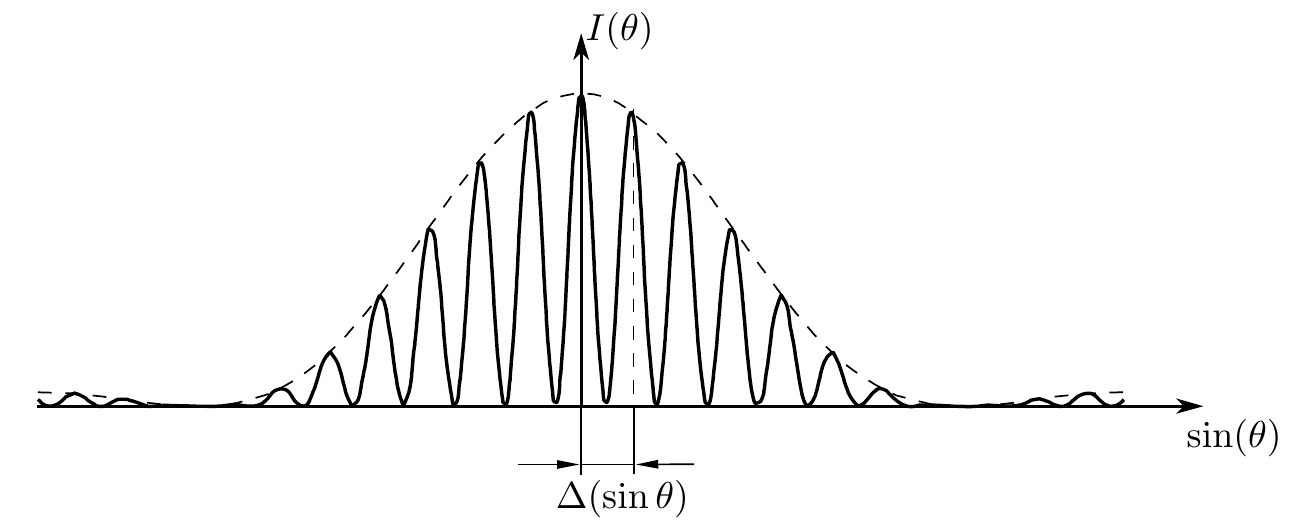
\includegraphics[width=0.8\linewidth]{../img/frau2.png}}
\end{figure}

\subsection{Дифракция Фраунгофера на решётке}
Рассмотрим периодическую структуру одинаковых щелей с периодом $d$. По аналогии с дифракцией на двух щелях запишем суммарный колебательный процесс в точке наблюдений как сумму колебаний от каждой щели с учётом сдвига фазы. Фаза колебаний от щели номер $m$ на $\alpha_m = m\alpha = -mkd\sin\theta$  отличается от фазы колебаний начальной щели. Если всего решётка имеет $N$ щелей, суммарное колебание в точке наблюдения есть
\[
g_N(\theta) = g(\theta) \sum_{m=0}^{N-1}e^{im\alpha}
\]

\begin{figure}[ht!]
    \center{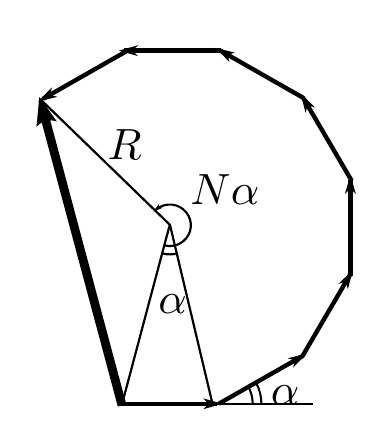
\includegraphics[width=0.4\linewidth]{../img/resh1.png}}
\end{figure}

Найдём сумму, построив векторную диаграмму. Каждое слагаемое $e^{im\alpha}$ изобразим вектором единичной длины, угол поворота которого относительно горизонтальной оси равен $m\alpha$. Получим цепочку вектором, показанную на рисунке.  Суммарное колебание изображается вектором, соединяющим начало и конец цепочки. Радиус окружности, в которую вписана цепочка векторов, равен $R=\frac{1}{2\left|\sin\alpha/2\right|}$, длина результирующего вектора равна $2R\left|\sin N\alpha/2\right|$. Отсюда получаем амплитуду колебания в точке наблюдения:
\[
    \left|g_N(\theta)\right| = \left|g(\theta)\right| \cdot \left|\frac{\sin{\frac{Nkd\sin\theta}{2}}}{\sin{\frac{kd\sin\theta}{2}}}\right|
\]
Распределение интенсивности $I(\theta) = \left|g_N(\theta)\right|^2$ по углам описывается формулой
\[
    I(\theta) = \left|g(\theta)\right|^2\left|\frac{\sin{\frac{Nkd\sin\theta}{2}}}{\sin{\frac{kd\sin\theta}{2}}}\right|^2
\]

Здесь первый сомножитель описывает картину дифракции на отдельной щели, а второй связан с интерференцией волн от разных щелей.


\begin{figure}[ht!]
    \center{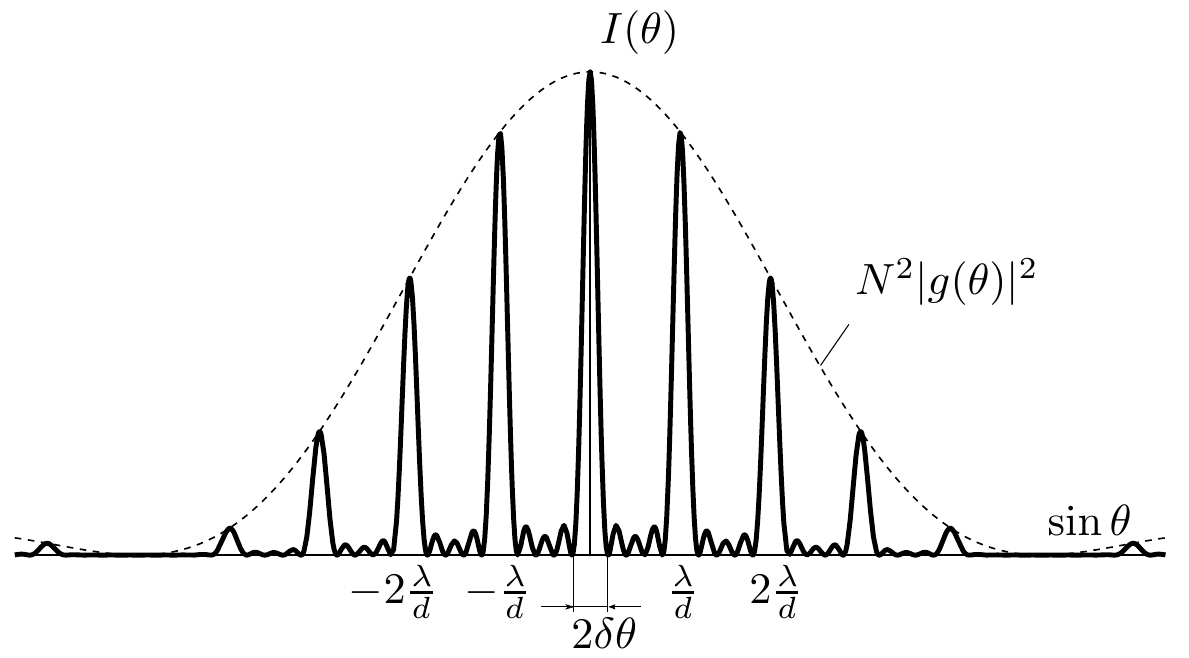
\includegraphics[width=0.8\linewidth]{../img/resh2.png}}
\end{figure}

Характерной особенностью решётки является наличие узких максимумов, в которые идёт подавляющая доля общего потока энергии. Их положения определяются условием
\[
d\sin\theta_m = m\lambda,
\]
означающим, что идущие в направлении $\theta_m$ волны от всех щелей складываются в одной фазе, так как при этом $-\alpha_m = kd\sin\theta_m = 2\pi m$. Поскольку фазы вкладов от всех щелей одинаковы, амплитуда колебаний в максимумах в $N$ раз больше амплитуды от одной щели, а интенсивность~--- в $N^2$.

Угловую полуширину максимумов $\delta\theta$ оценим, найдя ближайшую к  какому-либо $\theta_m$ точку $\theta = \theta_m + \delta\theta$, в которой функция обращается в нуль. Такая точка соответствует приращению аргумента синуса в числителе на $\pi$, то есть
\[
\delta(kd\sin\theta) = \frac{2\pi}{N}
\]
Для небольших углов оценка угловой полуширины главных дифракционных максимумов есть
\[
\delta\theta \approx \frac{\lambda}{Nd}
\]
Целое число $m$ называется порядком главного максимума. Максимальное значение $m$ ограничено величиной $d / \lambda$. Реально же заметными являются максимумы $m \le d / b$.

\subsection{Угловая дисперсия амплитудной решетки}
Угловая дисперсия $D(\lambda)$ характеризует угловое расстояние между близкими спектральными линиями:
\[
    D = \frac{d\varphi}{d\lambda} = \frac{m}{d\cos\varphi}=\frac{m}{\sqrt{d^2-m^2\lambda^2}}\approx \frac{m}{d}
\]

\subsection{Разрешающая способность амплитудной решетки}
Рассмотрим изображения спектра для двух узких спектральных линий с длинами волн $\lambda$ и $\lambda + \delta\lambda$. Для минимального значения $\delta\lambda$, которое может быть определено по результатам измерений, вводят важнейшую характеристику спектрального прибора~--- разрешающую способность:
\[
R = \frac{\lambda}{\delta\lambda}
\]
Решётку изготавливают с помощью делительной машины или методами литографии, далее её размножают или распечатывают. Копия эталонной решётки называется репликой. В учебных лаборато риях используются именно реплики. На большие решётки делительная машина наносит $10^4$--$10^5$ штрихов, шаг решётки составляет величину порядка микрометра. Если на одном участке решётки шаг чуть больше, а на других чуть меньше среднего, то в изображении спектра могут возникать ложные линии спектра. Они называются <<<духами>>>. Естественной причиной уменьшения разрешающей способности спектральных приборов является их старение и нарушение правил обращения с ними.

\begin{figure}[ht!]
    \center{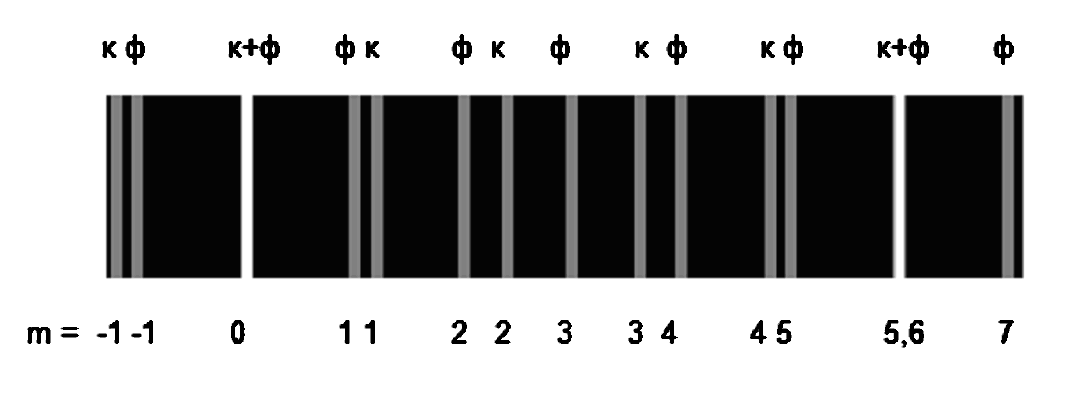
\includegraphics[width=0.8\linewidth]{../img/cyka.png}}
\end{figure}

Приведённые выше соображения относятся к техническим требованиям изготовления спектрального прибора. Рассмотрим физические ограничения разрешающей способности. На рисунке изображения спектральных линий являются изображениями входной щели коллиматора. Начнём уменьшать размер щели. В начале этого процесса будет уменьшаться интенсивность линий и их ширина. Начиная с некоторого момента будет уменьшаться только интенсивность, а ширина линий изменяться не будет. Достигнут физический предел ширины линии, и он определяется дифракцией света на апертуре решётки. Определим угловое расстояние между максимумом линии и её первым нулем~--- полуширину линии $\delta\varphi$. Пусть на решётку, состоящую из $N$ штрихов, падает параллельный пучок света перпендикулярно её поверхности. Если $N=2$, то две волны погасят друг друга, если между ними возникнет разность хода $\lambda / 2$, если $N = 3$, то $\lambda / 3$. В общем случае $N$ штрихов для полуширины линии $\delta\varphi$ получаем уравнение, решение которого при $\delta\varphi \ll 1$ имеет вид
\[
d\sin (\varphi_m + \delta\varphi) = m\lambda + \frac{\lambda}{N}
\]
\[
\delta\varphi = \frac{\lambda}{Nd\cos\varphi_m}
\]
$ND\cos\varphi_m$~--- видимый под углом $\varphi_m$ размер решётки. Угловое расстояние между двумя линиями определяется дисперсией
\[
\Delta\varphi \approx D\delta\lambda = \frac{m}{d\cos\varphi_m}\delta\lambda
\]

Для сравнения между собой различных спектральных приборов Релей предложил приравнять полуширину $\delta\varphi$ и расстояние между линиями $\Delta\varphi$. Критерий Релея удобен для различных оценок. Согласно ему для дифракционных решёток разрешающая способность определяется порядком спектра и числом штрихов:\
\[
R = Nm
\]
Здесь под $N$ следует понимать число одновременно работающих штрихов решётки, которое, вообще говоря, не равно суммарному числу штрихов освещённого участка решётки. Число штрихов $N$ определяется качеством реплики, размером источника света и т.д. Например, если источник является однородной линией шириной $b$ на расстоянии $z$ от решётки, то размер области решётки, засвеченной когерентно, определяется формулой $\rho \approx \lambda / \psi$, где $\psi = b / z$~--- угловой размер источника.

Основная числовая характеристика условия Релея — отношение интенсивности света в провале между линиями к максимальному значению. Численное значение этой характеристики для решетки равно $2\left(\frac{\sin\pi / 2}{\pi / 2}\right)^2 \approx 0{,}81$. В экспериментальной спектроскопии разрешающая способность спектрального прибора превосходит разрешение по критерию Релея при использовании вместо глаза малошумящих приемников света. Измеряется отношение ширины суммарной к ширине отдельной линиина уровне половинной мощности: для критерия Релея это отношение равно 2.

\subsection{Дисперсионная область амплитудной решетки}
При большой ширине спектра спектры различных порядков могут накладываться друг на друга. Предельная ширина спектрального интервала $\Delta \lambda$, при которой спектры соседних порядков перекрываются своими границами, называется дисперсионной областью. При этом $m(\lambda + \Delta\lambda) = (m+1)\lambda$ и
\[
\delta\lambda = \frac{\lambda}{m}
\]
